\documentclass[a4paper,12pt]{article}
\usepackage{graphicx}
\graphicspath{ {images/} }

%% Language and font encodings
\usepackage[utf8]{inputenc}
\usepackage[american]{babel}

% Specify bibliography package
\usepackage{csquotes}% Recommended
\usepackage[style=apa]{biblatex}
%\DeclareLanguageMapping{american}{american-apa}
\addbibresource{references.bib}

%% Sets page size and margins
\usepackage[top=2cm,bottom=2cm,left=2cm,right=2cm,marginparwidth=1.75cm]{geometry}
\setlength{\parskip}{1em}

%% package for formatting and highlighting source code
\usepackage{listings}
\usepackage{color}


%% Useful packages
\usepackage{amsmath}
\usepackage{graphicx}
\usepackage{float}
\usepackage[colorlinks=true, allcolors=black]{hyperref}
\usepackage{graphicx}
\usepackage{setspace}

% List of abbreviations
\usepackage{acronym}

% Section Title Margins
\usepackage{titlesec}
\titlespacing*{\section}
{0pt}{3.0ex plus 1ex minus .2ex}{0.7ex}
\titlespacing*{\subsection}
{0pt}{1.4ex}{0pt}

\definecolor{dkgreen}{rgb}{0,0.6,0}
\definecolor{gray}{rgb}{0.5,0.5,0.5}
\definecolor{mauve}{rgb}{0.58,0,0.82}

\lstset{frame=tb,
  language=Python,
  aboveskip=3mm,
  belowskip=3mm,
  showstringspaces=false,
  columns=flexible,
  basicstyle={\small\ttfamily},
  numbers=none,
  numberstyle=\tiny\color{gray},
  keywordstyle=\color{blue},
  commentstyle=\color{dkgreen},
  stringstyle=\color{mauve},
  breaklines=true,
  breakatwhitespace=true,
  tabsize=3
}
    
    
\title{Review of Assigned Readings}
\author{Your Name Goes Here}
        
    \begin{document}
    \begin{titlepage}
      	\begin{figure}
      	\centering
        
\includegraphics[scale=0.35]{logohsg}
        \end{figure}
        \centering
        School of Management, Economics, Law, Social Schiences and International Affairs \par
        \vspace{2.5cm}
        {\huge\bfseries The effect of Twitter activity on
Bitcoin price\par}      
        {\Huge\itshape Documentation\par}
        \vspace{1.5cm}     
        {Software Engineering for Economists \\ (7,610,1.00) \par}
        \vspace{1.3cm}
        {Dimitrios Koumnakes - 10-613-370 \\ Severin Kranz - 13-606-355 \\ Joël Sonderegger - 11-495-488 \\
       	Alen Stepic - 11-475-258 \\Chi Xu - XX-XXX-XXX \par}
        \vspace{1cm}
        Fall Term 2017
        \vfill
        Supervisor
        \linebreak
        Prof. Dr. Philipp \textsc{Zahn}
        \linebreak
        Department of Economics
          
    % Bottom of the page
     {\centering \today\par}
    
    \end{titlepage}
    
    \begin{abstract}
    \pagenumbering{Roman}
    \begin{spacing}{1.5}
    
  (Insert text)

    \end{spacing}
    
    \end{abstract}

    \clearpage
    \tableofcontents
    
    \clearpage
    
    \listoffigures 	
    \section*{List of Abbreviation} 
	\begin{acronym}[ASECRETTT] 
	\acro{API}{Application Programming Interface}
	\acro{ATOKEN}{Access Token}
	\acro{ASECRET}{Access Token Secret}
	\acro{CKEY}{Consumer Key}
	\acro{CSECRET}{Consumer Secret}
	\acro{JSON}{Java Script Object Notation}
	\acro{RPI}{Raspberry Pi}
	\acro{SSH}{Secure Shell}
	\end{acronym}
    \clearpage
    



\begin{spacing}{1.2}
\cleardoublepage\pagenumbering{arabic}
\section{Introduction}
In the academic environment accountability and reproducibility is important. However, the publishing process of papers and journals seem to be outdated. New ways of data collection and data processing exist by using computational economics. The usage of algorithms can increase effectiveness and efficiency. Hence, much lager data sets can be proceeded. However this creates also new problems regarding to traceability and reproducibility. Often cited academic paper exist, where the initial computation is not reproducible. Furthermore, some academic paper even contain computational errors. Replicating data or existing results do not provide any new knowledge at all. Nevertheless, the ability to reproduce increases trustworthiness and indicate the quality of the conducted work. This explains why reproduction is of great relevance.

\subsection{Goal of the paper}
The goal of this documentation is the provision of a description. This description should enable the reader to reproduce the results discussed in the separate paper. Thus, it contains an explanation how the input data have been gathered, stored, aggregated and analysed. In other words, the input data, the model core, the model parameters and the applied math program are explained.

\subsection{Methodology}
This documentation consists out of four chapters. The first chapter contains a short introduction and provides the reader with an overview about the topic. Furthermore it points out the relevance of documentation. The second chapter discusses the input data. This includes the process of gathering and storing twitter tweets as well as the gathering of the bitcoin price data. The third chapter discusses how the data is aggregated by pointing out the core model and its parameters. Finally the fifth chapter discusses how the analysis has been conducted.

\subsection{Scope}
The scope of the documentation is the provision of an overview about the different steps which have been conducted to obtain the results in the paper. It does not contain any discussions about the results of the separate paper. It is not a deep description of the code as the code itself as the code is documented separately. Nevertheless, important lines of code are discussed. 
\clearpage 


\section{Data Collection}
This section contains a detailed description of how the data for the sequential analysis is gathered and stored. This includes two  subsections the (1) tweets data and the (2) bitcoin price data.
\subsection{Tweets Data}
Whit the python script real-time twitter data are streamed and stored. This happens with help of a raspberry pi.
\subsubsection{Python Script}
Twitter offers different Application Programming Interfaces (API) for collecting data. However, the time frame for gathering data on a freely base is limited to 7 days. On the other hand, python offers different twitter libraries. Such as the open-source package tweepy. This package has been used for streaming the twitter data as it simplify the script.

\paragraph{Installing Tweepy}\mbox{}\\{}
Tweepy is installed very simply by running following commands in the command prompt. 
\begin{lstlisting}[language=bash]
pip install tweepy
\end{lstlisting}

If the previous downloaded python installation package does not contain the tweepy library, the tweepy package has to be downloaded. The package can be downloaded for free from the following link:
\begin{lstlisting}[language=bash]
https://pypi.python.org/pypi/tweepy
\end{lstlisting}

\paragraph{Twitter Authentication}\mbox{}\\{}
To access the twitter data, twitter requests an identification of the user. The identification is assured by different keys and access tokens. Those are the (1) consumer key (ckey), (2) consumer secret (csecret), (3) access token (atoken) and (4) access token secret (asecret).

To obtain the mentioned keys and tokens a twitter account is needed. Once, a twitter account exist a application has to be created. This has to be conducted by login with the twitter account credentials under the following link: 
\begin{lstlisting}[language=bash]
https://apps.twitter.com/
\end{lstlisting}

After the creation of a application, the keys and tokens can be extracted. Figure 1 illustrates how to retrieve the keys and tokens.
\begin{figure}[h]
\centering
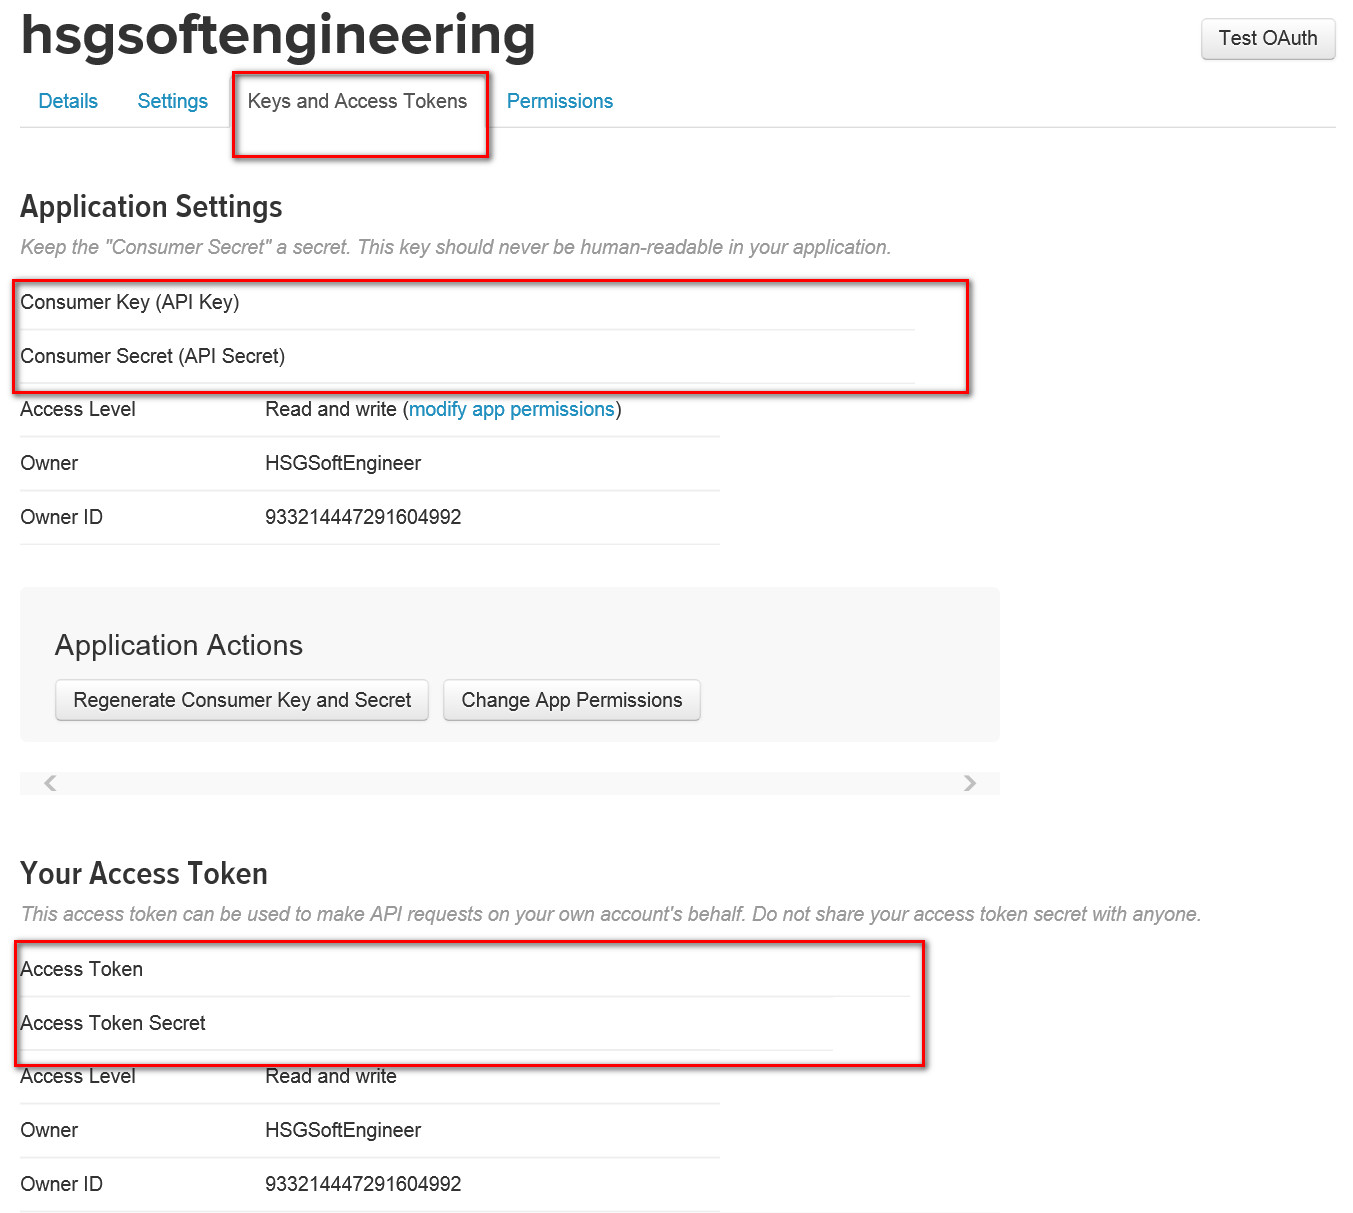
\includegraphics[scale=0.6]{twitteraccess}
\caption{Twitter Keys and Access Tokens}
\end{figure}

\paragraph{Twitter Streaming API}\mbox{}\\{}
By running the python script \verb|collectTwitterData.py| real-time twitter data is pushed in a Java Script Object Notation (JSON) format. Tweets are just pushed in case a tweet contains the defined key word \verb|bitcoin|.
\begin{lstlisting}[language=bash]
$ python collectTwitterData.py
\end{lstlisting}

From the JSON format the following parameters are decoded:
\begin{itemize}
    \item created at: Timestamp of the created tweet
    \item text: text of the tweet
\end{itemize}
The time timestamps are in UTC time.

After a successfully decoding the parameters the data is appended to the \verb|twitterData.csv| file in a new row and saved in the folder \verb|/data|.

An excerpt of an example response looks like the following:
\begin{lstlisting}
[
    {
        "created_at": Tue Dec 19 20:40:48 +0000 2017, 
        "text": "RT @WhiteBitcoin: New Bitcoin White. Effective, Flexible, Reliable", 
    }, 
    {
        "created_at": Tue Dec 19 20:40:49 +0000 2017 ,
        "text": "As #bitcoin prices surge, #xrp remains affordable and FAST!",
    }, 
    {
        "created_at": Tue Dec 19 20:40:49 +0000 2017, 
        "text": "Singapore issues bitcoin warning after price rise - #BTC #Bitcoin #Crypto", 
    }
]
\end{lstlisting}

Furthermore to ensure a high quality data set an exception has been integrated into the \verb|collectTwitterData.py| script. If an error occurs an email will be sent with the error message. Furthermore the logfile will be  appended to \verb|/data/tweet_collection_error_log.csv|.

\subsubsection{Hardware Setup}
As explained in the previous section the twitter API was used to filter tweets in realtime based on the buzzword "bitcoin". The python program was running for seven days without interruption on a Raspberry Pi 2 (RPI) which was accessed with a Secure Shell (SSH) connection. This approach allowed us to ensure a continuous data stream while being able to access the program output regardless anywhere and anytime. Furthermore due to a low energy consumption of the RPI the method is also the most cost efficient one compared to a personal computer or NAS Server. The following section describes the different steps that have been taken in order to setup the RPI 2, SSH, Git and Python3.\newline 

\begin{enumerate}
\item Setup of the Raspberry Pi
\begin{enumerate}
\item Burn image 2017-11-29-raspbian-stretch.zip to micro SD card available from
\begin{lstlisting}[language=bash]
https://www.raspberrypi.org/downloads/raspbian/
\end{lstlisting}
\item Boot image from micro SD card 
\item Open SSH session using PuTTY SSH client for Windows available from
\begin{lstlisting}[language=bash] 
https://www.chiark.greenend.org.uk/~sgtatham/putty/latest.html
\end{lstlisting}
\item Login to server with credentials 
\end{enumerate}

\item Update system to the newest software
\begin{enumerate}
\item Update list of applications with the command
\begin{lstlisting}[language=bash]
sudo apt-get update
\end{lstlisting}
\item Update applications with the command
\begin{lstlisting}[language=bash]
sudo apt-get upgrade
\end{lstlisting}
\end{enumerate}

\item Setup Git
\begin{enumerate}
\item Install Git using the command
\begin{lstlisting}[language=bash]
 sudo apt-get install git
\end{lstlisting}
\item Clone Git repository from
\begin{lstlisting}[language=bash] 
https://github.com/joelsonderegger/twitterbitcoin.git
\end{lstlisting}
\end{enumerate}

\item Setup Pyhton3
\begin{enumerate}
\item Install Python3 using the command: sudo apt-get install Python3 \newline
\item Install the tweepy module for python using the command
\begin{lstlisting}[language=bash]
pip install tweepy
\end{lstlisting}
\end{enumerate}

\item Collect Twitter Data
\begin{enumerate}
\item Open a new screen using the command
\begin{lstlisting}[language=bash] 
screen -S 'name' 
\end{lstlisting}
\item Start python program using the command
\begin{lstlisting}[language=bash]
python3 CollectTwitterData.py
\end{lstlisting}
\item Detach the screen to keep the program running after secure shell connection has been terminated using the commands
\begin{lstlisting}[language=bash]
Ctrl+A
Ctrl+D
\end{lstlisting}
\item Re-attach the screen to check whether the script is still running using the command
\begin{lstlisting}[language=bash]
screen -r 'name'
\end{lstlisting}
\end{enumerate}

\item Download the collected data
\begin{enumerate}
\item Install FileZilla available from
\begin{lstlisting}[language=bash] 
https://filezilla-project.org/
\end{lstlisting}
\item Connect to rpi and navigate to data location \newline
\item Download data manually \newline \newline \end{enumerate}
\end{enumerate}
In summary, this approach worked well and ran smoothly. A clean setup is recommended to ensure a continuous data stream over a longer period.


\subsection{Bitcoin Price Data}
We wrote a Python script which collects Bitcoin price data as there was no preexisting data set that satisfied our needs. The Bitcoin price is best expressed by the Bitcoin Price Index. The Bitcoin price index (BPI) is an index of the exchange rate between the Bitcoin (BTC) and the US dollar (USD) (\cite{kristoufek2015main}). The objective of the script was to gather hourly Bitcoin Price Index data for at least the time period in which we gather the tweets data. We found the an API by bitcoinaverage.com which sufficed our needs. An API description follows later.

\subsubsection{Execution}
By executing the python script \verb|collectCryptocurrencyData.py| hourly data for the Bitcoin Price Index is retrieved.
\begin{lstlisting}[language=bash]
    $ python collectCryptocurrencyData.py
\end{lstlisting}

\subsubsection{Output}
After successfully running the python script \verb|CollectCryptocurrencyData.py| the file \verb|bpi.csv| is generated in the folder \verb|/data|. It is important to note that every execution of the script overwrites any existing \verb|bpi.csv| file.

The file \verb|bpi.csv| contains historical Bitcoin Price Index data for one month on an hourly basis. Each data point consists of the following parameters:
\begin{itemize}
    \item time: Timestamp on an hourly basis in UTC time
    \item average: Average price (in USD)
    \item high: Highest price (in USD)
    \item low: Lowest price (in USD)
    \item open: Opening price (in USD)
\end{itemize}

\subsubsection{API: Bitcoinaverage.com}
Bitcoinaverage.com offers a free API that provides real-time and historical price data for a range of crypto-currencies including Bitcoin. The following requests delivers data for an per hour monthly sliding window.
\paragraph{Request}\mbox{}\\
The request to get the data for an per hour monthly sliding window looks as follows. This request require authentication that requires registration and the generation of an API key. The registration and generation of an API key is freely available on bitcoinaverage.com. The collectCryptocurrencyData.py already contains the necessary keys. This means that you need no register or generate keys to execute the script collectCryptocurrencyData.py.  
\begin{lstlisting}[language=bash]
https://apiv2.bitcoinaverage.com/indices/global/history/BTCUSD?period=monthly&?format=json
\end{lstlisting}
\paragraph{Response}
An excerpt of an example response looks like the following:
\begin{lstlisting}
[
    {
        "high": 8271.04, 
        "average": 8247.83, 
        "open": 8242.39,
        "low": 8217.72, 
        "time": "2017-11-22 15:00:00"
    }, 
    {
        "high": 8246.82,
        "average": 8203.19,
        "open": 8203.81,
        "low": 8157.25,
        "time": "2017-11-22 14:00:00"
    }, 
    {
        "high": 8267.27, 
        "average": 8238.62, 
        "open": 8248.77, 
        "low": 8198.54, 
        "time": "2017-11-22 13:00:00"
    }
]
\end{lstlisting}


\section{Data Aggregation and Data Wrangling}
Before the collected data sets can be analyzed they need to be aggregated. In addition, some data wrangling is necessary to bring the data in a format which than can be analyzed. 

\subsubsection{Execution}
By executing the python script \verb|aggregateTwitterBpi.py| a aggregated data set that contains number of tweets and Bitcoin Price Index, both on an hourly basis, gets generated. 
\begin{lstlisting}[language=bash]
    $ python aggregateTwitterBpi.py
\end{lstlisting}

\subsubsection{Output}
After successfully running the python script \verb|aggregateTwitterBpi.py| the file \verb|nr_of_tweets_bpi_closing_price.csv| is generated in the folder \verb|/data|. It is important to note that every execution of the script overwrites any existing \verb|nr_of_tweets_bpi_closing_price.csv| file.

The file \verb|aggregateTwitterBpi.csv| contains historical tweets and Bitcoin Price Index data. Each data point consists of the following parameters:
\begin{itemize}
    \item time: Timestamp on an hourly basis in UTC time
    \item {nr\_of\_tweets}: 
    \item {df\_nr\_of\_tweets}: 
    \item {log\_df\_nr\_of\_tweets}: 
    \item {df\_bpi\_closing\_price}: 
    \item {log\_df\_bpi\_closing\_price}: 
\end{itemize}


\section{Data Analysis}
(Dimitri's Part)

\end{spacing}
\clearpage

%************************** Bibliography **************************
\printbibliography
\clearpage

%************************** DOCUMENT-END **************************
\end{document}